\documentclass[../functional_analysis.tex]{subfiles}
\begin{document}
\section{Aula 10 - 11 de Setembro, 2025}
\subsection{Motivações}
\begin{itemize}
	\item Conjuntos de Primeira e Segunda Categorias;
	\item Teorema Categórico de Baire e Consequências
\end{itemize}
\subsection{Transformações Lineares Ilimitadas}

Nosso próximo tópico de estudo será alguns fatos elementares sobre as transformações lineares, não necessariamente limitadas.

Sejam X, Y espaços vetoriais normados sobre um mesmo corpo \(\mathbb{K}\) e \(A:D(A)\subseteq X\rightarrow Y\), uma transformação linear, onde D é um subespaço vetorial de X.

Definiremos alguns conceitos relacionados às transformações lineares que usaremos de notação:

\begin{def*}
	Para a transformação linear \(A:X\rightarrow Y\), diremos que:
	\begin{itemize}
		\item \(D(A)\) denotará o \textbf{domínio de A};
		\item \(\mathrm{Graf}(A) = \{(u, Au)\in X\times Y:\; u\in D(A)\}\subseteq X\times Y\) é o \textbf{gráfico de A};
		\item \(\mathrm{Im}(A)=\{Ax\in Y:\; x\in D(A)\}\) é a \textbf{imagem de A}; e
		\item \(N(A) = \mathrm{ker}(A) = \{x\in D(A):\; Ax = 0\}\) é o \textbf{núcleo de A}.
	\end{itemize}
	Além disso, se \(D(A)\) é denso em X, diremos que A é \textbf{densamente definida}. \(\square\)
\end{def*}

\begin{example}
	Seja \(X = \mathcal{C}([0, 1], \mathbb{R})\) com a norma usual, \(D(A) = \mathcal{C}^{1}([0, 1], \mathbb{R})\) e defina
	\begin{align*}
		A: & D(A)\subseteq X\rightarrow X                             \\
		   & u\longmapsto (Au)(s) = u'(s), \quad \forall s\in [0, 1].
	\end{align*}
	Note que esta transformação linear não é limitada!
\end{example}

\begin{def*}
	Uma transformação linear A é dita \textbf{fechada} se seu gráfico
	\[
		\mathrm{Graf}(A) = \{(x, A(x)): x\in X,\; A(x)\in Y\} \subseteq X\times Y
	\]
	é fechado em \(X\times Y.\; \square\)
\end{def*}
Uma consequência da definição é que
\begin{prop*}
	Seja \(A:D(A)\subseteq X\rightarrow X\) uma transformação linear. Então, A é fechada se, e somente se, para toda sequência \(\{(u_{n}, Au_{n})\}\) em \(D(A)\times Y\) que é convergente em \(X\times Y\) para algum \((u, v)\in X\times Y\), temos
	\[
		u\in D(A) \quad\&\quad Au = v.
	\]
\end{prop*}


Lembre-se que uma transformação linear \(A:D(A)\subseteq X\rightarrow Y\) é limitada se existe uma constante \(c\geq 0\) tal que
\[
	\Vert Au \Vert\leq c\Vert u \Vert,\quad \forall u\in D(A).
\]
Se A é limitada e densamente definida, podemos estendê-la a uma transformação linear limitada definida em X; neste caso, veremos, como consequência do \hyperlink{closed_graphic}{\textit{Teorema do Gráfico Fechado}}, que A não é fechada, a não ser que \(D(A) = X.\)

Além disso, provaremos que, como outra consequência do \hyperlink{closed_graphic}{\textit{Teorema do Gráfico Fechado}} que se X e Y forem espaços de Banach e \(A:X\rightarrow Y\) for uma transformação linear fechada, então A é limitada. Já temos um contraexemplo do caso em que X e Y não são de Banach, pois a transformação do exemplo anterior é fechada, mas ilimitada.

Apesar disso, em geral, estamos apenas interessados em estudar transformações lineares fechadas definidas entre espaços de Banach X, Y. Assim, as únicas transformações lineares fechadas \(A:D(A)\subseteq X\rightarrow Y\) que não são limitados estão definidos em um subespaço vetorial \(D(A)\subsetneq X\).

\begin{def*}
	Diremos que uma transformação linear A é \textbf{fechável} se \(\overline{\mathrm{Graf}(A)}\) é gráfico de uma transformação linear; neste caso, \(\overline{\mathrm{Graf}(A)}\) define uma transformação linear \(\overline{A}: D(\overline{A})\subseteq X\rightarrow Y\) e \(D(A)\subseteq D(\overline{A})\), com
	\[
		Au = \overline{A}u,\quad \forall u\in D(A).\; \square
	\]
\end{def*}
Da definição acima, segue que \(\overline{A}\) em si é fechada e que ela é a menor extensão fechada de A.

De forma análoga à proposição acima,
\begin{prop*}
	Seja \(A:D(A)\subseteq X\rightarrow Y\) uma transformação linear; então, A é fechável se, e somente se, para toda sequência \(\{(u_{n}, Au_{n})\}\) em \(D(A)\times Y\) que é convergente para \((0, v)\in X\times Y\), temos \(v=0.\)
\end{prop*}
\begin{proof*}
	Denotemos por \(\overline{A}\) a transformação linear tal que
	\[
		\mathrm{Graf}(\overline{A}) = \overline{\mathrm{Graf}(A)}
	\]
	e suponha que A é fechável com fecho \(\overline{A}\). Se \(\{u_{n}\}\) é uma sequência em \(D(A)\) que converge para zero e tal que \(\{Au_{n}\}\) é convergente com limite v, devemos ter
	\[
		0=\overline{A}0 = v.
	\]

	Por outro lado, suponha que, para toda sequência \(\{(u_{n}, Au_{n})\}\) em \(D(A)\times Y\) que é convergente para \((0, v)\) em \(X\times Y\), temos \(v = 0\). Se \((u, v),\; (u, \overline{v})\in \overline{\mathrm{Graf}(A)}\), existem sequências \(\{(u_{n}, Au_{n})\}\) e \(\{(\overline{u_{n}}, A \overline{u_{n}})\}\) tais que
	\[
		(u_{n}, Au_{n})\rightarrow (u, v) \quad\&\quad (\overline{u_{n}}, A \overline{u_{n}})\rightarrow (u, \overline{v})
	\]
	em \(X\times Y.\) Desta forma, \(u_{n}-\overline{u_{n}}\) é um ponto no domínio de A, e
	\[
		(u_{n}-\overline{u_{n}}, A(u_{n}-\overline{u_{n}}))\rightarrow (0, v-\overline{v}),
	\]
	levando à conclusão de que \(v=\overline{v}.\) Logo, \(\overline{\mathrm{Graf}(A)}\) é gráfico de um transformação linear. Portanto, o resultado segue. \qedsymbol
\end{proof*}
Em todas as aplicações de interesse, A é fechável com domínio denso.
\subsection{Teorema Categórica de Baire}
\begin{def*}
	Se \((X, \rho )\) for um espaço métrico, um conjunto \(A\subseteq X\) será \textbf{nunca denso} ou \textbf{raro} se o seu fecho tiver interior vazio, ou seja,
	\[
		\mathrm{int}{(\overline{A})} = \emptyset .\; \square
	\]
\end{def*}
\begin{def*}
	Um conjunto \(A\subseteq X\) será de \textbf{primeira categoria em X} se for a união enumerável de conjuntos nunca densos; caso contrário, ele será dito de \textbf{Segunda Categoria em X.} \(\square\)
\end{def*}
Consequentemente,
\begin{prop*}
	Um espaço métrico \((X, \rho )\) será de segunda categoria nele mesmo se, e somente se, em qualquer representação de X como união enumerável de fechados, pelo menos um deles contém uma bola aberta.
\end{prop*}
Além disso, ganhamos o
\hypertarget{baire_theorem}{
	\begin{theorem*}[Teorema Categórico de Baire]
		Todo espaço métrico completo é de segunda categoria nele mesmo.
	\end{theorem*}
}

\begin{proof*}
	Suponha que não, ou seja, que
	\[
		X = \bigcup_{i=1}^{\infty}F_{i}
	\]
	com cada \(F_{i}\) fechado e de interior vazio; então, o conjunto \(X\setminus{F_1}\) é não vazio e aberto.

	Seja \(x_1\) e \(0 < \varepsilon_1 < 1\) tais que
	\[
		x\in X\setminus{F_1}\quad\&\quad B_{\varepsilon_1}(x_1)\cap F_1 = \emptyset .
	\]
	Como
	\[
		B_{\frac{\varepsilon_1 }{2}}\subsetneq F_2,
	\]
	existe \(x_2\) neste conjunto e \(\varepsilon_2 < 1/2\) tais que
	\[
		B_{\varepsilon_2}(x_2)\cap F_2 = \emptyset \quad\&\quad B_{\varepsilon_2}(x_2)\subseteq B_{\frac{\varepsilon_1}{2}}(x_1).
	\]
	Indutivamente, existe \(x_{n}\) e \(\varepsilon_{n} < 2^{-(n-1)}\) tais que
	\[
		x_{n}\in B_{\frac{\varepsilon_{n-1}}{2}}(x_{n-1}),\; B_{\varepsilon_{n}}(x_{n})\cap F_{n} = \emptyset ,\;\&\; B_{\varepsilon_{n}}(x_{n})\subseteq B_{\frac{\varepsilon_{n-1}}{2}}(x_{n-1}).
	\]
	\begin{figure}[H]
		\begin{center}
			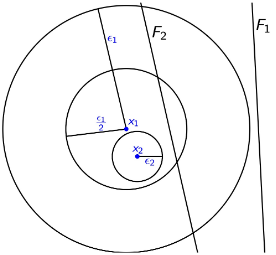
\includegraphics[height=0.4\textheight, width=0.4\textwidth, keepaspectratio]{./Images/b2_10.png}
		\end{center}
		\caption{A bolinha está sem pontos em comum com \(F_1\), mas tem com \(F_2\). O processo indutivo resulta na imagem abaixo:}
	\end{figure}
	\begin{figure}[H]
		\begin{center}
			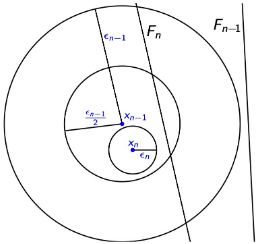
\includegraphics[height=0.4\textheight, width=0.4\textwidth, keepaspectratio]{./Images/bn_10.png}
		\end{center}
	\end{figure}

	Consequentemente, a sequência \(\{x_{n}\}\) é de Cauchy, pois, para cada k natural,
	\[
		x_{n+k}\in B_{\frac{\varepsilon_{n}}{2}}(x_{n})
	\]
	e \(\varepsilon_{n}\) converge para 0 conforme n tende a infinito; logo, como X é completo, \(\{x_{n}\}\) é convergente.

	Suponha que x é este limite; para cada n fixo, \(x\in B_{\varepsilon_n}(x_{n})\), justamente pois os \(x_{n+k}\)'s pertencem a cada bola de raio \(\varepsilon_{n}/2\) centrada em \(x_{n}\). Portanto,
	\[
		x\not\in \bigcup_{n=1}^{\infty}F_{n} = X,
	\]
	que é uma contradição. \qedsymbol

\end{proof*}
\begin{example}
	Todo espaço de Banach é de segunda categoria nele mesmo.
\end{example}
\begin{def*}
	Sejam \(X, Y\) espaços vetoriais normados e \(T:X\rightarrow Y\) uma transformação linear.
	\begin{itemize}
		\item[1)] Diremos que T será \textbf{aberta} se \(T(U)\) for aberto em Y, sempre que U for aberto em X; e
		\item[2)] Diremos que T será \textbf{fechada} se \(\mathrm{Graf}(T) = \{(x, Tx):\; x\in X\}\) for fechado em \(X\times Y\).
	\end{itemize}
\end{def*}
Um teorema muito importante da análise correlaciona as aplicações abertas com os conjuntos de segunda categoria, conhecido como
\hypertarget{open_application}{
	\begin{theorem*}[Teorema da Aplicação Aberta]
		Seja X um espaço de Banach e Y um espaço vetorial normado. Se \(T\in \mathcal{L}(X, Y)\) e \(T(X)\) for de segunda categoria em Y, entãp:
		\begin{itemize}
			\item[a)] T será sobrejetora;
			\item[b)] T será aberta; e
			\item[c)] Y será de segunda categoria.
		\end{itemize}
	\end{theorem*}
}
\begin{crl*}
	Sejam X e Y espaços de Banach.
	\begin{itemize}
		\item[1)] Se \(T\in \mathcal{L}(X, Y)\) for sobrejetora, então T será aberta; e
		\item[2)] Se \(T\in \mathcal{L}(X, Y)\) for bijetora, então T será um isomorfismo.
	\end{itemize}
\end{crl*}

\end{document}
